\chapter{Акт о~внедрении результатов диссертационной работы}\label{app:act}

Результаты диссертационной работы внедрены и~используются в~деятельности
ФГБУ <<НИЦ <<Институт имени Н.\,Е.\,Жуковского>>>> в~работах
по~автоматическому распознаванию и~реидентификации объектов. Применение
разработанного методического и~программного обеспечения подтверждено
актом о~внедрении, скан-копия которого приведена ниже.

\begin{figure}[htbp]
\centering
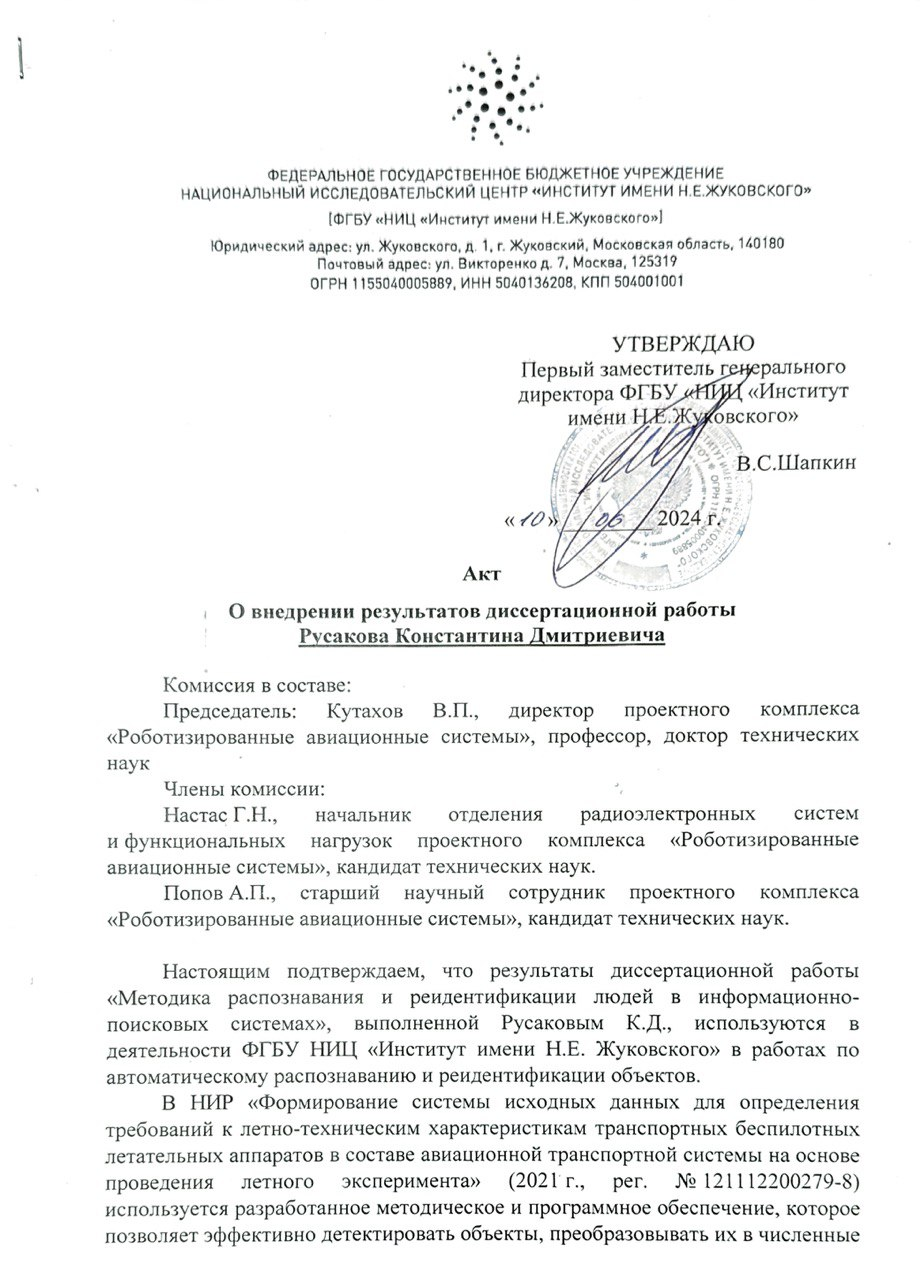
\includegraphics[width=0.85\textwidth,height=0.85\textheight,keepaspectratio]{images/act-impl-1.jpg}
\caption{Акт о~внедрении результатов диссертационной работы (страница~1)}
\label{fig:app/act-1}
\end{figure}

\begin{figure}[htbp]
\centering
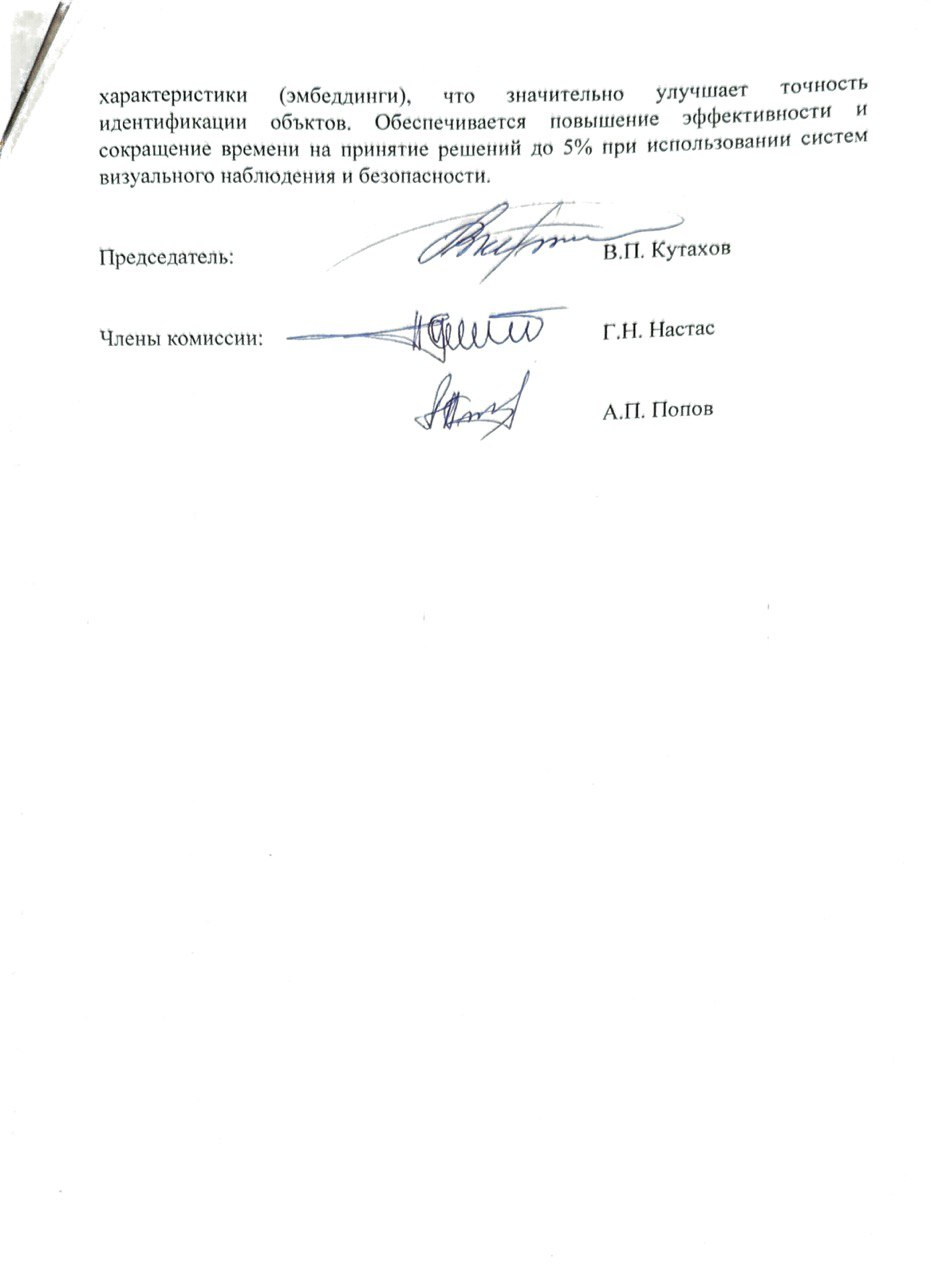
\includegraphics[width=0.85\textwidth,height=0.85\textheight,keepaspectratio]{images/act-impl-2.jpg}
\caption{Акт о~внедрении результатов диссертационной работы (страница~2)}
\label{fig:app/act-2}
\end{figure}

\clearpage

\chapter{Свидетельства о~государственной регистрации программ для~ЭВМ}\label{app:reg}

В~ходе выполнения диссертационной работы разработанные программные
средства защищены свидетельствами о~государственной регистрации
программ для~ЭВМ Федеральной службы по~интеллектуальной собственности
(Роспатент). Скан-копии свидетельств приведены ниже.

\begin{figure}[htbp]
\centering
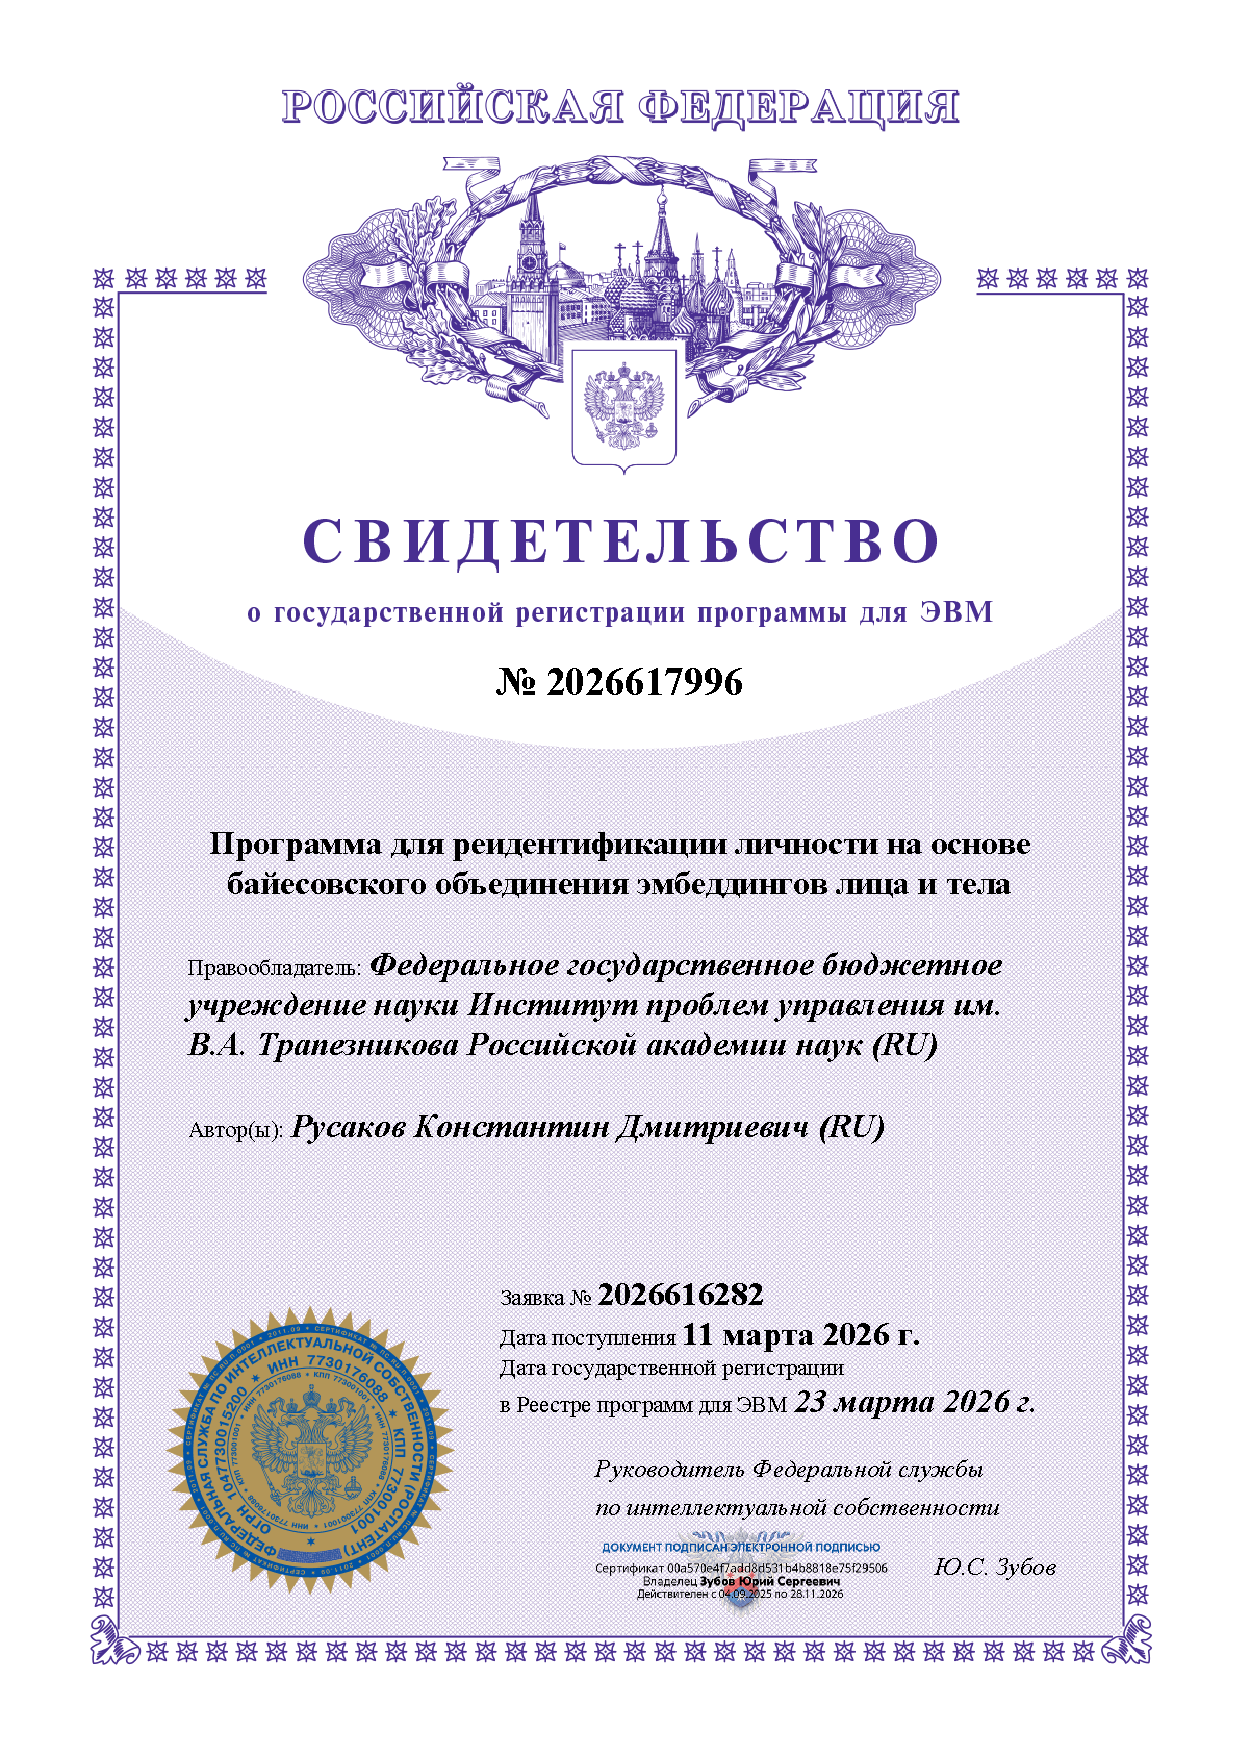
\includegraphics[width=0.85\textwidth,height=0.85\textheight,keepaspectratio]{images/prog-2026617996.pdf}
\caption{Свидетельство о~государственной регистрации программы для~ЭВМ
№\,2026617996 от~23.03.2026 <<Программа для реидентификации личности
на~основе байесовского объединения эмбеддингов лица и~тела>>}
\label{fig:app/prog-2026617996}
\end{figure}

\begin{figure}[htbp]
\centering
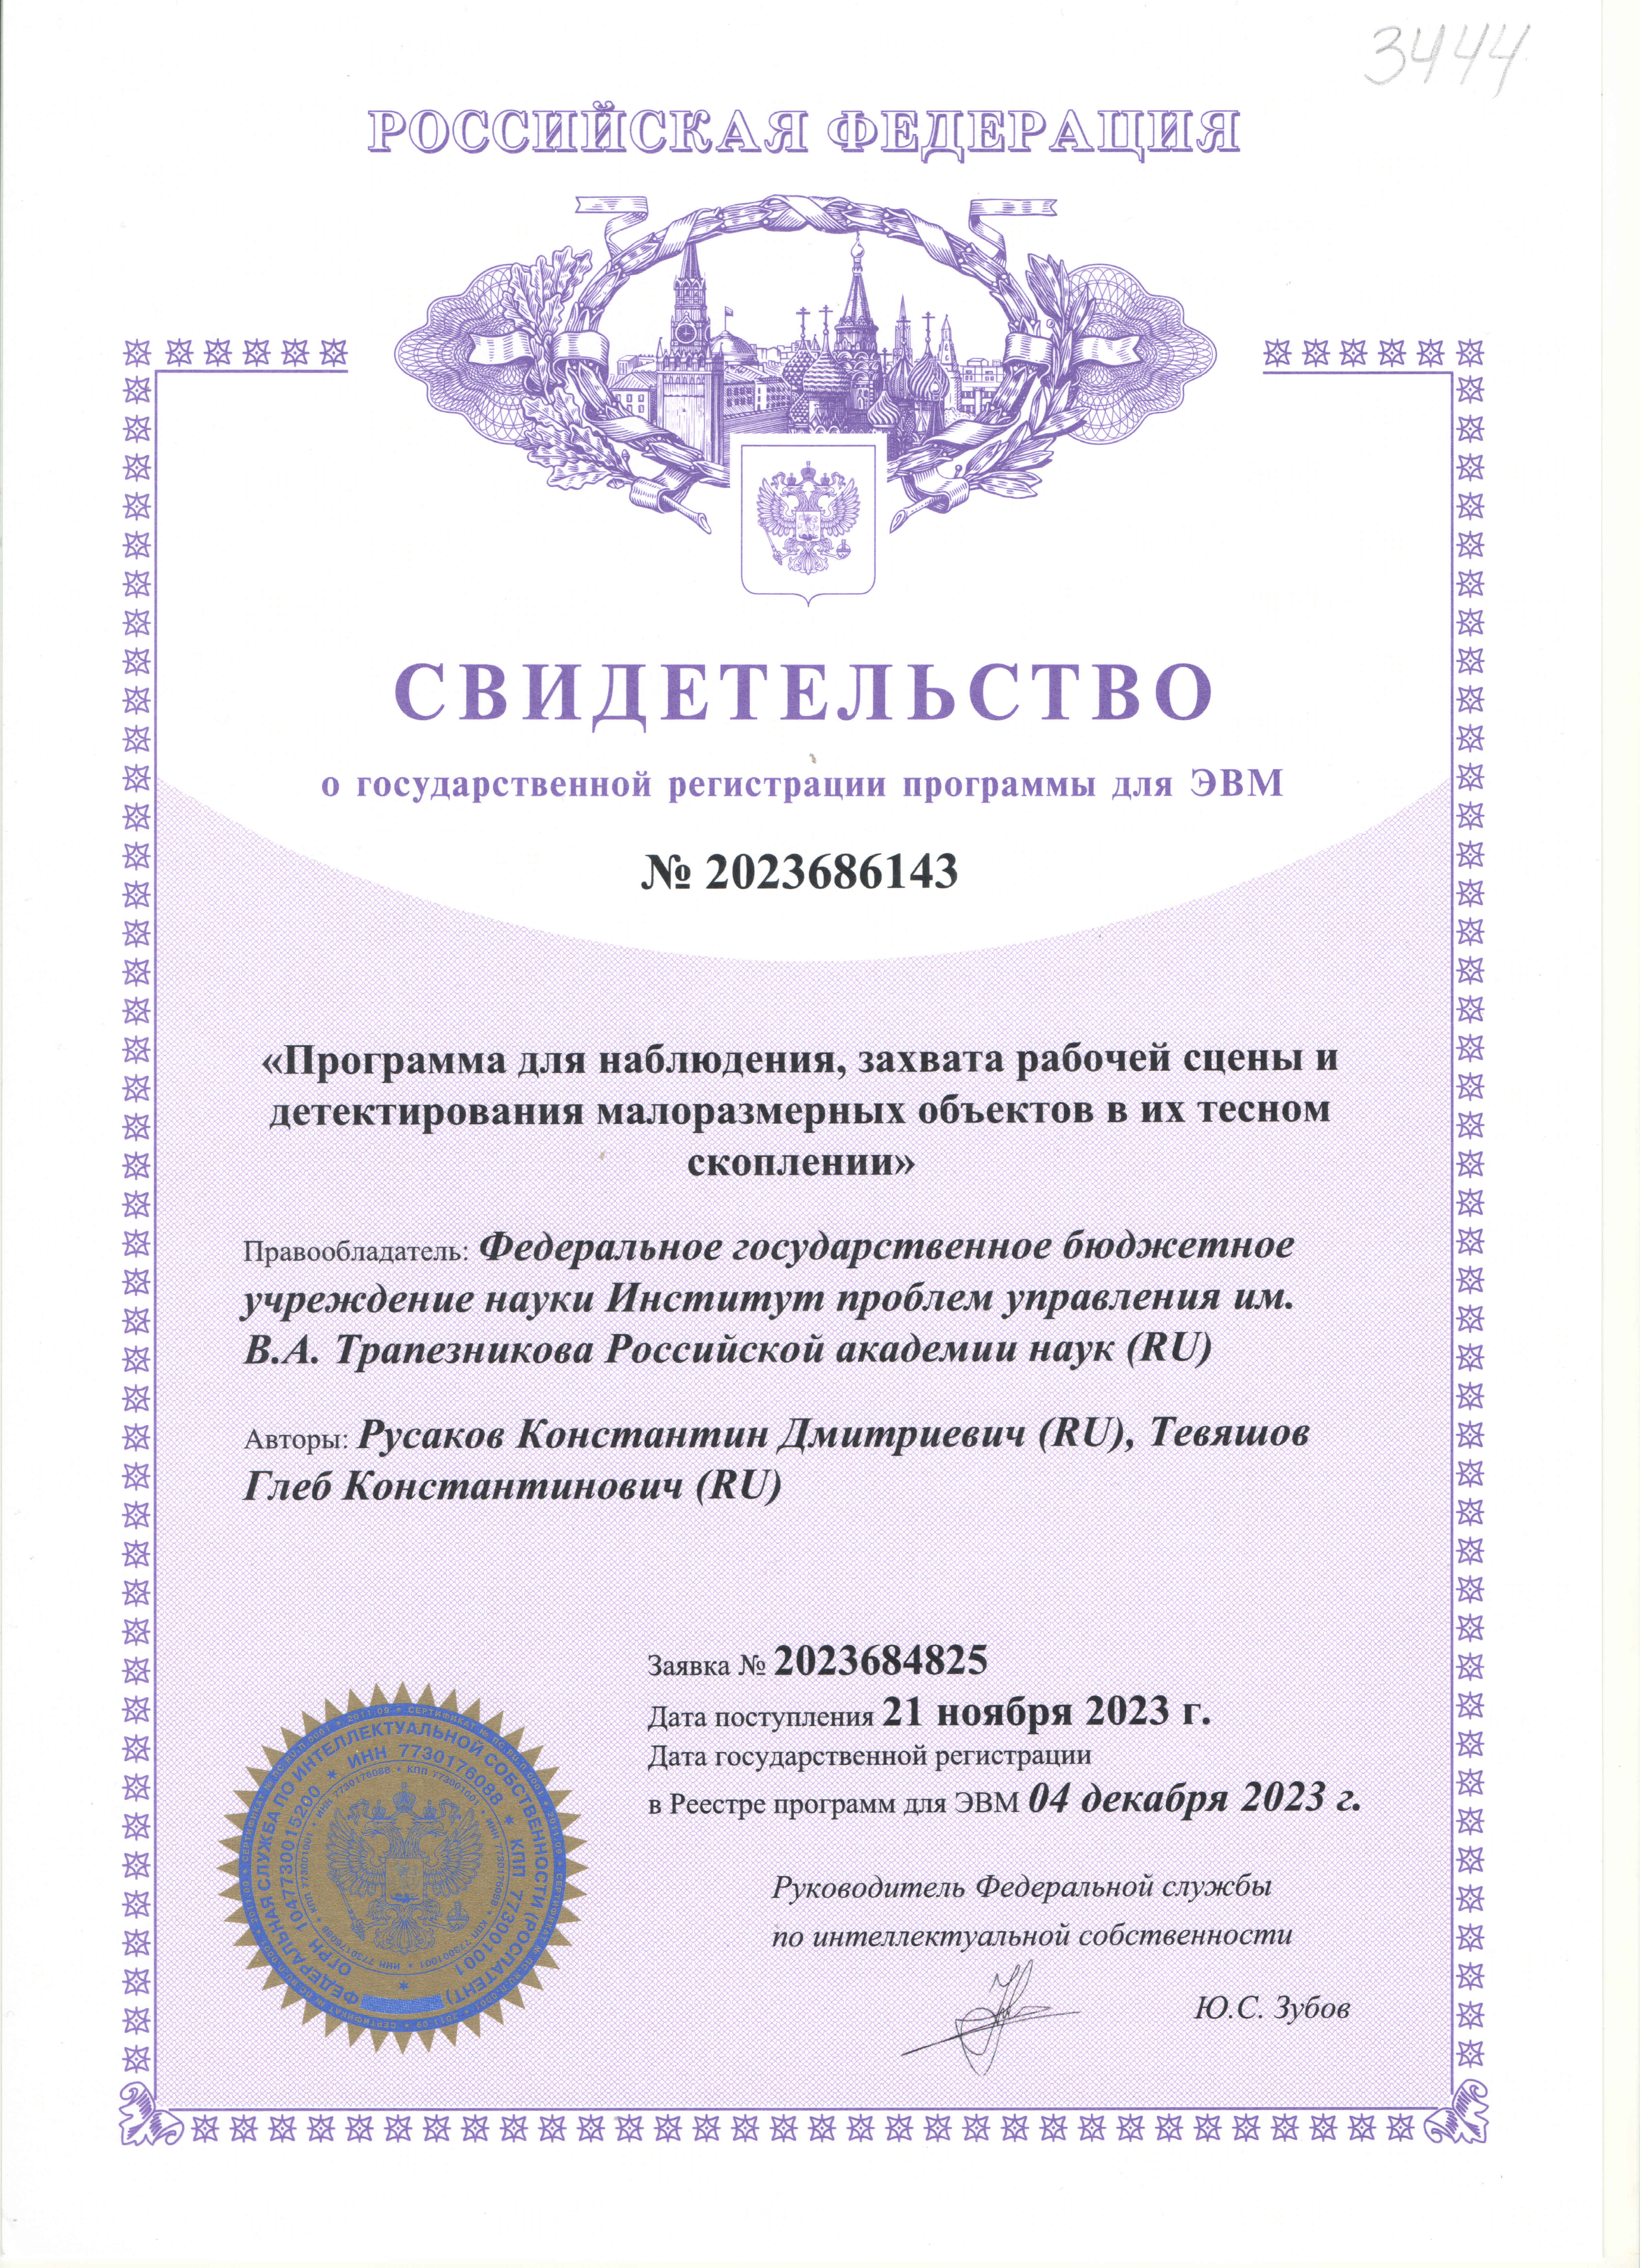
\includegraphics[width=0.85\textwidth,height=0.85\textheight,keepaspectratio]{images/prog-2023686143.jpg}
\caption{Свидетельство о~государственной регистрации программы для~ЭВМ
№\,2023686143 от~04.12.2023 <<Программа для наблюдения, захвата рабочей
сцены и~детектирования малоразмерных объектов в~их тесном скоплении>>}
\label{fig:app/prog-2023686143}
\end{figure}

\clearpage

\chapter{Исходный код программы для~ЭВМ}\label{app:code}

В~настоящем приложении приведен полный исходный код программы для~ЭВМ
<<Программа для реидентификации личности на~основе байесовского
объединения эмбеддингов лица и~тела>> (свидетельство о~государственной
регистрации №\,2026617996 от~23.03.2026, файл
\texttt{bayesian\_reid\_system.py}). Программа реализует комплексную
методику, описанную в~главах~\ref{ch:ch2} и~\ref{ch:ch3}, и~является
официально зарегистрированным программным продуктом, обеспечивающим
воспроизводимость экспериментальной части работы.

\begingroup
\lstset{
    language=Python,
    basicstyle=\scriptsize\ttfamily,
    numbers=left,
    numberstyle=\tiny\color{Gray},
    stepnumber=10,
    breaklines=true,
    breakatwhitespace=true,
    showstringspaces=false,
    columns=fullflexible,
    frame=single,
    framerule=0.3pt,
    rulecolor=\color{Gray},
    aboveskip=0.5em,
    belowskip=0.5em,
    keywordstyle=\color{Mahogany}\bfseries,
    commentstyle=\color{ForestGreen}\itshape,
    stringstyle=\color{Brown},
}
\lstinputlisting{bayesian_reid_system_listing.py}
\endgroup

